\documentclass[aspectratio=169,10pt]{beamer}
\usepackage{booktabs}
\usepackage{tikz}
\usetikzlibrary{positioning,arrows.meta}

\usetheme{default}
\setbeamertemplate{navigation symbols}{}
\setbeamertemplate{footline}[frame number]
\setbeamertemplate{itemize items}[circle]
\definecolor{accent}{RGB}{0,90,160}
\definecolor{muted}{RGB}{95,95,95}
\setbeamercolor{frametitle}{fg=accent}
\setbeamercolor{structure}{fg=accent}
\setbeamerfont{frametitle}{series=\bfseries,size=\large}
\newcommand{\hl}[1]{\textcolor{accent}{\textbf{#1}}}
\newcommand{\head}[1]{\textbf{#1}\par\smallskip}

% TODO: fill in the three team members' names.
\newcommand{\team}{[Name 1], [Name 2], [Name 3]}

\begin{document}

% ---------------------------------------------------------------- slide 1
\begin{frame}{Improving the Compute Efficiency of Puro-2B}
{\small\color{muted} Project proposal \,·\, Speedrun Topic 1 \,·\, \team}
\medskip

\begin{columns}[T,onlytextwidth]
\begin{column}{0.56\textwidth}
\head{Motivation}
Puro-2B trains a Qwen2-1.5B-level model from scratch on RTX~5090 GPUs for
about \$6.9K. Every further saving makes LLM pretraining research more
accessible to small labs.

\medskip
\head{Problem}
Reach the same downstream quality with \hl{30\% less compute}.

\medskip
{\small
\begin{tabular}{@{}lcc@{}}
\toprule
 & Puro-2B & Our target \\
\midrule
Avg.\ score, 15 benchmarks & 57.81 & $\ge 57.81$ \\
RTX 5090 GPU-hours & 22{,}514 & $\le 15{,}760$ \\
\bottomrule
\end{tabular}}
\end{column}
\begin{column}{0.40\textwidth}
\head{Key observation}
Puro-2B sees 1.4T tokens with 2B parameters: about
\hl{700 tokens per parameter}.

\medskip
The paper itself calls this an overtrained, data-rich regime. The model is
limited by its \emph{capacity}, not by data.

\medskip
$\Rightarrow$ Spend fewer FLOPs on each token, and give the model more
capacity to absorb the data.
\end{column}
\end{columns}
\end{frame}

% ---------------------------------------------------------------- slide 2
\begin{frame}[t]{Method: sparse capacity (MoE) at lower cost per token}
\begin{columns}[T,onlytextwidth]
\begin{column}{0.52\textwidth}
\head{Main idea: replace each MLP with a mixture of experts}
\begin{itemize}\setlength{\itemsep}{2pt}
\item MLPs are $\approx 60\%$ of Puro-2B's FLOPs per token
      {\small\color{muted}(our estimate)}.
\item 16 experts, each $\tfrac18$ of the MLP width ($2\times$ capacity);
      every token uses its top-$k$.
\item $k = 4,\,3,\,2$ $\Rightarrow$ \hl{$\approx 30\%,\ 38\%,\ 45\%$ fewer
      FLOPs per token}.
\item Margin: at $k=2$ we save $\ge 30\%$ GPU-hours even if MoE layers
      run at half the dense throughput.
\end{itemize}

\smallskip
\head{Fallback: fewer tokens, better data mixture}
{\small Halving Phase-2 tokens costs only $\approx 0.45$ points in the
paper. A 30\% cut made this way needs $\approx 0.3$--$0.5$ points back,
which we seek by re-weighting data sources (RegMix).}
\end{column}
\begin{column}{0.44\textwidth}
\centering
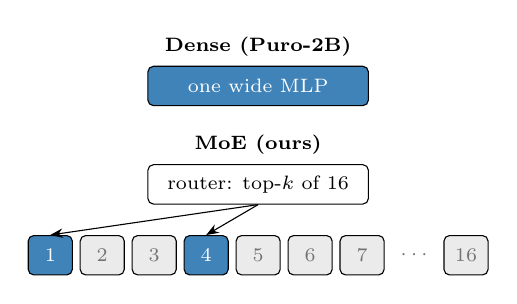
\begin{tikzpicture}[
  font=\scriptsize,
  box/.style={draw, rounded corners=2pt, minimum height=5mm, inner sep=2pt},
  on/.style={box, fill=accent!75, text=white},
  off/.style={box, fill=black!8, text=black!55},
  >={Stealth[length=1.6mm]}]
  \node[font=\scriptsize\bfseries] at (0,2.05) {Dense (Puro-2B)};
  \node[on, minimum width=28mm] at (0,1.55) {one wide MLP};
  \node[font=\scriptsize\bfseries] at (0,0.8) {MoE (ours)};
  \node[box, minimum width=28mm] (r) at (0,0.3) {router: top-$k$ of 16};
  \foreach \i/\s/\l in {1/on/1,2/off/2,3/off/3,4/on/4,5/off/5,6/off/6,7/off/7,9/off/16}{
    \node[\s, minimum width=5.6mm] (e\i) at ({-3.3+0.66*\i},-0.6) {\l};
  }
  \node[text=black!55] at ({-3.3+0.66*8},-0.6) {$\cdots$};
  \draw[->] (r.south) -- (e1.north);
  \draw[->] (r.south) -- (e4.north);
\end{tikzpicture}

\smallskip
\raggedright
\head{How we measure}
{\small
\begin{enumerate}\setlength{\itemsep}{1pt}
\item Throughput: MoE layer vs.\ dense MLP.
\item Proxy models on H100: validation loss at equal tokens
      ($\ge 200$ tokens per parameter).
\item Metric: \hl{5090 GPU-hours to reach the dense baseline's loss}.
\end{enumerate}}
\end{column}
\end{columns}
\end{frame}

% ---------------------------------------------------------------- slide 3
\begin{frame}[t]{First experiments and expected results}
\begin{columns}[T,onlytextwidth]
\begin{column}{0.58\textwidth}
\head{Step 1: throughput test (no training)}
Time the MoE layer against the dense MLP at Puro-2B's sizes for
$k = 2, 3, 4$; on H100 now, on RTX~5090 once we have access.

\medskip
\head{Step 2: quality at proxy scale (H100)}
{\footnotesize\setlength{\tabcolsep}{3pt}
\begin{tabular}{@{}lll@{}}
\toprule
 & \textbf{E0: dense baseline} & \textbf{E1: MoE} \\
\midrule
Layers / hidden & 12 / 768 & 12 / 768 \\
MLP & width 2304 & 16 experts $\times$ 288, top-$k$ \\
Active MLP width & 2304 & 576 / 864 / 1152 \\
Data, optimizer & \multicolumn{2}{l}{same Puro data, same MuonH recipe} \\
Training tokens & \multicolumn{2}{l}{equal, $\ge 200$ per parameter} \\
\bottomrule
\end{tabular}}

\smallskip
\textbf{Question:} what is the smallest $k$ that matches E0's validation
loss?

\medskip
{\small\textbf{Status:} Puro's training stack runs on the course H100
cluster on Puro data that we tokenized ourselves.}
\end{column}
\begin{column}{0.385\textwidth}
\head{Expected results}
\begin{itemize}\setlength{\itemsep}{2pt}
\item $k = 2$ or $3$ matches E0, also at larger proxies (0.6B, 1.7B).
\item \hl{$\ge 30\%$ fewer GPU-hours} at equal loss. This needs MoE layers
      at $\ge 50\%$ of dense speed for $k=2$, or $\ge 75\%$ for $k=3$.
\item If MoE falls short, we fall back on fewer tokens plus a better data
      mixture.
\end{itemize}

\smallskip
\head{Main risks}
{\small
\begin{itemize}\setlength{\itemsep}{1pt}
\item Experts may be too slow on 5090.
\item More parameters must fit in 32\,GB.
\item Proxies may not transfer to 2B.
\end{itemize}}
\end{column}
\end{columns}
\end{frame}

\end{document}
